
\documentclass[10pt,a4paper,titlepage]{article}
\usepackage[english]{babel}
\usepackage[utf8]{inputenc}
\usepackage[margin=100pt]{geometry}


\usepackage{graphicx}   % Import pictures
\usepackage{ragged2e}   % fullfill paragraphs
%\usepackage{multicol}
%\usepackage{lscape}
\usepackage{xcolor}
%\usepackage{listings}
\usepackage{courier}
\usepackage{caption}

\usepackage[backend=biber, sorting=none]{biblatex}
\addbibresource{dokumentace.bib}



\begin{document}
%-----------------------------------------%
%	            TITLE PAGE                %
%-----------------------------------------%
\begin{titlepage}

\begin{center}
% Headings
\textsc{\LARGE Brno University of technology}\\[0.5cm]
\textsc{\large Faculty of Information Technology}\\[8cm]

% Title - lines
{ \huge \bfseries DHCP Starvation attack}\\[0.3cm]
{ \Large \bfseries Project documentation}\\[0.5cm]
{ \bfseries Martin Benes}\\

\end{center}

\end{titlepage}
\newpage

%-----------------------------------------%
%	              DOCUMENT                  %
%-----------------------------------------%

\pagenumbering{gobble}

The task of the project was to gather informations about DHCP protocol and
afterwards write a program in C, that performs a DHCP starvation attack.



\section*{DHCP}


\subsection*{Motivation}
Every private network manages its own IP address space with reserved addresses, that
can be given to the internal devices. An assignment of the addresses may be
done either manually or automatically, using DHCP agent.

Manual configuration forces the network administrator to manually setup the
local address for every device, newly connected to the network.

The more pleasant way, especially for administrator, is using {\it plug-and-play}
DHCP protocol, where the address assignment is done by DHCP server.
\cite{computernetworking} \cite{pocitacovesite}



\subsection*{DHCP protocol}

\begin{figure}[h!]
    \begin{center}
        \includegraphics[width=0.18\textwidth]{dhcpcomm.png}
        \caption{ DHCP communication. \label{fig:triangle} \cite{DHCPcomm}}
    \end{center}
\end{figure}

When a device shows up in the network, it has not any local address, yet
it may communicate via broadcast.

\subparagraph{DHCP Discovery}
The device has to inform DHCP server about itself. The DHCP server does not have
any strict local address, so the device sends DHCP Discovery packet to the
broadcast address ff.ff.ff.ff, which is received by every device in the
network, including the DHCP server.

\subparagraph{DHCP Offer}
The server then reserves an address for the device, and sends DHCP Offer
response, unicast or multicast (set in received DHCP Discovery). If the
unicast is used, the MAC address from the DHCP Discovery is used as target
address (on L2).

\subparagraph{DHCP Request}
The DHCP client (the device) then sends DHCP Request to the server (again
it must be to the broadcast address, the local address is not assigned yet).
The client may receive several DHCP Offer packets (there might be more DHCP
servers in the network), but when the servers receives the DHCP Request from
the client, answering another server, they will withdraw the offer and return
the reserved address back to the address pool.

\subparagraph{DHCP Acknowledgement}
After receiving the DHCP Request, the server sends DHCP Acknowledgement,
including address lease duration. \cite{mistrovstvivsitich} \cite{DHCPwikipedia}
\cite{IPKDHCP}



\subsection*{DHCP Attack variants}

\paragraph{DHCP Discovery flood}
The clients sends repeatedly a large number of DHCP Discovery attacks with 
randomly generated MAC address (in {\it chaddr}). As a result, the DHCP server will
offer the whole pool using {\it DORA}\footnote{DHCP Discover - DHCP Offer - DHCP
Request - DHCP Acknowledgement packet sequence.} process, so the new legitimate
clients will not obtain an IP addresses from DHCP address.

In WPA 2 (IEEE 802.11), a client connection includes an association with AP
(Access Point) and session key generation, where the client's MAC address is used.
The AP has a maximal number of addresses it can associate, which prevents
the pool from exhaustion.

This may be solved with using different MAC address in ethernet header and
DHCP header. The ethernet header (read by AP) uses client's real MAC, so
it is forwarded, because it is already associated. The DHCP header than includes
the randomly generated MAC address.

On the other hand, the DORA process will not be completed, so the DHCP pool
will not get literally starved. 

\paragraph{Induced DHCP starvation}
In this type of attack, there are three parties, a victim, a client, who wants to
acquire an IP from a server, the server, that assigns IP addresses and an
attacker, that listens to the communication using {\it eavesdropping}. 

The client and the server do the classic DORA process, without any interrogation
of the attacker listening. After that, the client sends ARP\_REQ broadcast packet
checking the assigned IP address. The source IP address is still set to 0.0.0.0,
because the client still does not have the configured IP yet.

The attacker then reacts with ARP\_REPLY, which is received by the client.
The destination IP address of the packet is 0.0.0.0.

The malicious client sends DHCP Decline to the server to avoid the IP conflict,
because it is convinced, that the IP address received from the DHCP server
has already been assigned (to the attacker).

The server marks the IP address as unvailable for a lease period. The victim starts
the whole procedure repeateadly until the pool is fully unavailable.
\cite{IBSattack} \cite{DHCPstarvation}



\subsection*{Security mechanisms}

\paragraph{Port security}
The simpliest way, how to prevent such attacks is limitation of MAC addresses
per port in a network switch. If the limit is reached, the incident is reported
from a agent (switch) to the manager as SNMP trap.

This check is applicable to the DHCP Discovery flood attack, where the MAC address
in the L2 is randomly generated, but is not, if the different MAC addresses are used.

\paragraph{DHCP snooping}
This type of mechanism checks the matching MAC address in ethernet header
and in {\it chaddr} in DHCP header, it can detect the attack, where the MAC
addresses differ.

\paragraph{Dynamic ARP inspection}
DAI uses DHCP snooping check and creates a database of records {\it MAC address
- IP address - VLAN interface}. It is filled with scanned DHCP communication
of the client with a DHCP server.

It is able to detect, if the senders MAC address and IP address, acquired from
the DHCP server in the previous DORA communication, are the same as in
incoming packet. If not so, the fake ICMP communication is recognized as not
valid and the actions against it are taken.



\newpage
\printbibliography

\end{document}